\documentclass[12pt, a4paper, oneside]{ctexart}
\usepackage{minted, multicol, geometry, graphicx, fancyvrb, amssymb}
\usepackage{relsize, setspace, enumitem, float, hyperref, amsmath}

\geometry{a4paper, scale = 0.85}

\setenumerate[1]{itemsep=0pt,partopsep=0pt,parsep=\parskip,topsep=0pt}
\setitemize[1]{itemsep=0pt,partopsep=0pt,parsep=\parskip,topsep=0pt}
\setdescription{itemsep=0pt,pa
rtopsep=0pt,parsep=\parskip,topsep=0pt}
\setlength{\parindent}{0pt}

\setminted[cpp]{
	style=xcode,
	mathescape,
	linenos,
	autogobble,
	baselinestretch=1,
	tabsize=3,
	fontsize=\scriptsize,
	%bgcolor=Gray,
	frame=single,
	framesep=1mm,
	framerule=0.3pt,
	numbersep=1mm,
	breaklines=true,
	breaksymbolsepleft=2pt,
	%breaksymbolleft=\raisebox{0.8ex}{ \small\reflectbox{\carriagereturn}}, %not moe!
	%breaksymbolright=\small\carriagereturn,
	breakbytoken=false,
	% showtabs=true,
	% tab={\relscale{0.6} $\big\vert \ \ \ $ \relscale{1}},
}

\setminted[bash]{
    style=xcode,
	mathescape,
	linenos,
	autogobble,
	baselinestretch=1,
	tabsize=3,
	fontsize=\scriptsize,
	frame=single,
	framesep=1mm,
	framerule=0.3pt,
	numbersep=1mm,
	breaklines=true,
	breaksymbolsepleft=2pt,
	breakbytoken=false,
}

\title{ACM 模板}
\author{钱智煊,黄佳瑞,车昕宇}
\date{\today}

\begin{document}
    \scriptsize
    \maketitle
    \newpage
    
    \begin{multicols}{2}
        \tableofcontents
        \newpage

        \section{做题指导}
        \subsection{上机前你应该注意什么}
        \begin{enumerate}
    \item 预估你需要多少机时,以及写出来以后预计要调试多久,并在纸上记下。
    \item 先想好再上机,不要一边写一边想。
    \item 如果有好写的题,务必先写好写的。
    \item 把题目交给擅长的人来写,而不是空闲的人。
\end{enumerate}
        \subsection{机上你应该注意什么}
        \begin{enumerate}
    \item 机时应充分利用,手速应快一些。
    \item 如果你遇到了问题(做法假了、需要分讨等),先下机并通知队友。不要占着机时想。
    \item 建议使用整块时间写题,尽量不要断断续续的写。
\end{enumerate}
        \subsection{交题前你应该注意什么}
        \begin{enumerate}
    \item \verb|long long| 开了没有。
    \item 数组开够没有。
    \item 多测清了没有。
    \item 边界数据 \verb|(corner case)| 考虑了没有
    \item 调试输出删了没有
\end{enumerate}
编译命令:
\inputminted{bash}{src/tools/compile.sh}
        \subsection{如果你的代码挂了}
        按照优先级列出:
\begin{enumerate}
    \item 先 P 再下机。(P 还没有送来就分屏调。)
    \item 看 \verb|long long| 开了没有,数组开够没有,多测清了没有。
    \item 检查 typo ,你有没有打错一些难蚌的地方。
    \item 看看你题读错没有。
    \item 检查你的代码逻辑,即你的代码实现是否与做法一致。同时让另一个人重新读题。
    \item 怀疑做法假了。拉一个人一起看代码。
\end{enumerate}

        \section{图论}
        \subsection{tarjan}
        \subsubsection{有向图缩点}
        \inputminted{cpp}{src/graph/tarjan-directed.cpp}
        \subsubsection{无向图求割点}
        \inputminted{cpp}{src/graph/tarjan-vertex.cpp}
        \subsubsection{无向图求桥}
        \inputminted{cpp}{src/graph/tarjan-edge.cpp}
        \subsubsection{构建圆方树}
        将点双连通分量定义为不含割点的联通图。

将原图中的点称作圆点,而每个点双对应一个方点。将每个圆点向其所在的所有点双对应方点连边,就得到了圆方树。

特别的,仅含一条边的图也是点双(因其不含割点),这保证了圆方树的连通性。

\begin{figure}[htbp]
    \centering
    \includegraphics[width=0.8\textwidth]{https://pic.imgdb.cn/item/66d46de3d9c307b7e9acf664.png}
    \caption{圆方树示意图}
\end{figure}

圆方树会建立很多新的点,所以不要忘记\textbf{给数组开两倍!}

\begin{minted}{cpp}
void tarjan(int u)
{
    dfn[u]=low[u]=++Time,sta[++tp]=u;
    for(int v:G[u])
    {
        if(!dfn[v])
        {
            tarjan(v),low[u]=min(low[u],low[v]);
            if(low[v]==dfn[u])
            {
                int hav=0; ++All;
                for(int x=0;x!=v;tp--) x=sta[tp],T[x].pb(All),T[All].pb(x),hav++;
                T[u].pb(All),T[All].pb(u),;
                siz[All]=++hav;
            }
        }
        else low[u]=min(low[u],dfn[v]);
    }
}
\end{minted}
        \subsubsection{2-SAT}
        2-sat 问题定义为:给定 $m$ 个布尔表达式,每个包含两个布尔变量,形如 $a\lor b$ 。求是否存在一种赋值方式,使得所有表达式都为真。

对于表达式 $a\lor b$ ,显然若 $a$ 假则 $b$ 必真,反之亦然。因此,考虑将每个变量拆为两个点,分别代表此变量取值为真或假。对于每个表达式 $a\lor b$ ,连边 $\neg a\to b$ 与 $\neg b\to a$ 。对于边 $u\to v$ ,意义为若 $u$ 为真则 $v$ 必为真。那么对于最后得到的图,如果同一变量拆出的点处在同一强连通分量中,则无解,因为在可行解中它们的取值必然是不同的,但同一强连通分量中的点取值必然相同;否则,考虑缩点以后得到的 DAG ,取其拓扑序,对于每一个变量,令其取拆出的拓扑序较大的点对应的值即可。特别的,以上的判定是必要的,但我还不知道怎么证明它是充分的。
        \subsection{欧拉路径}
        欧拉图的判定:考虑起点、终点与中间点的必要条件即可。可以证明必要条件也是充分的。
以下给出已确定起点的无向图欧拉路径(回路)的构造算法。
\inputminted{cpp}{src/graph/euler-path.cpp}
        % \subsection{斯坦纳树}
        \subsection{网络流}
        \subsubsection{最大流(dinic)}
        \inputminted{cpp}{src/graph/dinic.cpp}
        \subsubsection{最小费用最大流(dinic)}
        \inputminted{cpp}{src/graph/mcmf-dinic.cpp}
        \subsubsection{最小费用最大流(edmonds-karp)}
        \inputminted{cpp}{src/graph/mcmf-ek.cpp}
        \subsubsection{无源汇有上下界可行流}
        \inputminted{cpp}{src/graph/feasible-bounded-flow.cpp}
        \subsubsection{有源汇有上下界最大流}
        \inputminted{cpp}{src/graph/max-bounded-flow.cpp}
        % \subsubsection{最小割树}

        \section{数据结构}
        \subsection{平衡树}
        \subsubsection{无旋 Treap}
        \inputminted{cpp}{src/data structure/fhq.cpp}
        \subsubsection{平衡树合并}
        如果需要合并两个有交集的 Treap 时该怎么做?我们可以每次将较小的数合并到较大的树中去,这样每个点最多只会合并 $\log n$ 次,每次合并复杂度 $O(n\log n)$,总时间复杂度 $O(n\log n\log V)$。

代码其实非常暴力,就是直接对更小的那棵树直接一个个插入进去:

\inputminted{cpp}{src/data structure/treap-merge.cpp}

\href{https://codeforces.com/blog/entry/108601}{可以证明},若只支持合并与分裂操作,则时间复杂度为 $O(n\log n)$ 。
        \subsubsection{Splay}
        \inputminted{cpp}{src/data structure/splay.cpp}
        \subsection{动态树}
        \inputminted{cpp}{src/data structure/LCT.cpp}
        \subsection{珂朵莉树}
        \inputminted{cpp}{src/data structure/ODT.cpp}
        \subsection{李超线段树}
        \subsubsection{修改与询问}
        \inputminted{cpp}{src/data structure/lichao.cpp}
        \subsubsection{合并}
        \inputminted{cpp}{src/data structure/lichao-merge.cpp}
        \subsection{二维树状数组}
        \inputminted{cpp}{src/data structure/2D-BIT.cpp}
        \subsection{虚树}
        \inputminted{cpp}{src/data structure/virtual-tree.cpp}
        \subsection{左偏树}
        \inputminted{cpp}{src/data structure/heap.cpp}
特别的,若要求给定节点所在左偏树的根,须使用并查集。对于每个节点维护 rt[] 值,查找根时使用函数:
\begin{minted}{cpp}
int find(int x) { return rt[x] == x ? x : rt[x] = find(rt[x]); }
\end{minted}
在合并节点时,加入:
\begin{minted}{cpp}
rt[x] = rt[y] = merge(x, y);
\end{minted}
在弹出最小值时加入:
\begin{minted}{cpp}
rt[ls(x)] = rt[rs(x)] = rt[x] = merge(ls(x), rs(x));
\end{minted}
另外,删除过的点是不能复用的,因为这些点可能作为并查集的中转节点。
        \subsection{吉司机线段树}
        \begin{itemize}
    \item 区间取 min 操作:通过维护区间次小值实现,即将区间取 min 转化为对区间最大值的加法,当要取 min 的值 v 大于次小值时停止递归。时间复杂度通过标记回收证明,即将区间最值视作标记,这样每次多余的递归等价于标记回收,总时间复杂度为 $O(m\log n)$。
    \item 区间历史最大值:通过维护加法标记的历史最大值实现。
\end{itemize}
\inputminted{cpp}{src/data structure/seg-beats.cpp}
        \subsection{树分治}
        熟知序列分治的过程是选取恰当的分治点并考虑所有跨过分治点的区间。而树分治的过程也是类似的,以点分治为例,每一次选择当前联通块的重心作为分治点,然后考虑所有跨越分治点的路径,并对分割出的联通块递归。

若要处理树上邻域问题,可以考虑建出点分树。处理点 x 的询问时,只需考虑 x 在点分树上到根的路径,每一次加上除开 x 所在子树的答案即可。

\inputminted{cpp}{src/data structure/tree-divide.cpp}
        % 关于扫描线。
        % 线段树优化建图没有必要。
        % 线段树分治没有必要。
        % 莫队的奇偶优化(看情况)
        % 笛卡尔树计数(为什么要写这种东西)
        % 树分块。
        % 树状数组上二分。
        % ETT 。
        % cdq 以及其它分治。
        % 莫队。

        % exchange argument 。
        
        \section{字符串}
        \subsection{后缀数组(与后缀树)}
        \inputminted{cpp}{src/string/SA.cpp}
        \subsection{AC自动机}
        \inputminted{cpp}{src/string/ACAM.cpp}
        \subsection{回文自动机}
        \inputminted{cpp}{src/string/PAM.cpp}
        \subsection{Manacher算法}
        \inputminted{cpp}{src/string/manacher.cpp}
        \subsection{KMP算法与border理论}
        \inputminted{cpp}{src/string/kmp.cpp}
字符串的border理论:
以下记字符串 $S$ 的长度为 $n$ 。
\begin{itemize}
    \item 若串 $S$ 具备长度为 $m$ 的 border ,则其必然具备长度为 $n-m$ 的周期,反之亦然。
    \item 弱周期性引理:若串 $S$ 存在周期 $p$ 、$q$ ,且 $p+q\le n$ ,则 $S$ 必然存在周期 $\gcd(p,q)$ 。
    \item 引理1:若串 $S$ 存在长度为 $m$ 的 border $T$,且 $T$ 具备周期 $p$ ,满足 $2m-n\ge p$ ,则 $S$ 同样具备周期 $p$ 。
    \item 周期性引理:若串 $S$ 存在周期 $p$ 、$q$ ,满足 $p+q-\gcd(p,q)\le n$ ,则串 $S$ 必然存在周期 $\gcd(p,q)$ 。
    \item 引理2:串 $S$ 的所有 border 的长度构成了 $O(\log n)$ 个不交的等差数列。更具体的,记串 $S$ 的最小周期为 $p$ ,则其所有长度包含于区间 $[n \bmod p + p, n)$ 的 border 构成了一个等差数列。
    \item 引理3:若存在串 $S$ 、$T$ ,使得 $2|T|\ge n$ ,则 $T$ 在 $S$ 中的所有匹配位置构成了一个等差数列。
    \item 引理4:PAM 的失配链可以被划分为 $O(\log n)$ 个等差数列。
\end{itemize}
        \subsection{Z函数}
        Z函数用于求解字符串的每一个后缀与其本身的 lcp 。其思路和 manacher 算法基本一致,都是维护一个扩展过的最右端点和对应的起点,而当前点要么暴力扩展使最右端点右移,要么处在记录的起点和终点间,从而可以利用已有的信息快速转移。
\inputminted{cpp}{src/string/zfunc.cpp}
        \subsection{后缀自动机}
        字符串 $S$ 的 SAM 是一个接受 $S$ 的所有后缀的最小 DFA 。例如 $S=\text{abbb}$ 的 SAM 如下:
\begin{figure}[H]
    \centering
    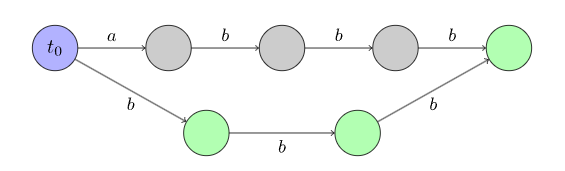
\includegraphics[width=0.45\textwidth]{src/string/SAM.png}
    \label{sam}
\end{figure}
SAM 的后缀链接构成了原串的后缀树。

对于代码实现,首先,我们实现一种存储一个转移的全部信息的数据结构。如果需要的话,你可以在这里加入一个终止标记,也可以是一些其它信息。我们将用一个 map 存储转移的列表,允许我们在总计 $O(n)$ 的空间复杂度和 $O(n\log |\Sigma|)$ 的时间复杂度内处理整个字符串。
\begin{minted}{cpp}
struct state {
    int len, link;
    std::map<char, int> next;
};
\end{minted}
SAM 本身将会存储在一个 \verb|state| 结构体数组中。我们记录当前自动机的大小 \verb|sz| 和变量 \verb|last| ,当前整个字符串对应的状态。
\begin{minted}{cpp}
const int MAXLEN = 100000;
state st[MAXLEN * 2];
int sz, last;
\end{minted}
我们定义一个函数来初始化 SAM(创建一个只有初始状态的 SAM)。
\begin{minted}{cpp}
void sam_init() {
    st[0].len = 0;
    st[0].link = -1;
    sz++;
    last = 0;
}
\end{minted}
最终我们给出主函数的实现:给当前行末增加一个字符,对应的在之前的基础上建造自动机。
\begin{minted}{cpp}
void sam_extend(char c) {
    int cur = sz++;
    st[cur].len = st[last].len + 1;
    int p = last;
    while (p != -1 && !st[p].next.count(c)) {
        st[p].next[c] = cur;
        p = st[p].link;
    }
    if (p == -1) {
        st[cur].link = 0;
    } else {
        int q = st[p].next[c];
        if (st[p].len + 1 == st[q].len) {
            st[cur].link = q;
        } else {
            int clone = sz++;
            st[clone].len = st[p].len + 1;
            st[clone].next = st[q].next;
            st[clone].link = st[q].link;
            while (p != -1 && st[p].next[c] == q) {
                st[p].next[c] = clone;
                p = st[p].link;
            }
            st[q].link = st[cur].link = clone;
        }
    }
    last = cur;
}
\end{minted}

        \section{线性代数}
        \subsection{高斯消元}
        \inputminted{cpp}{src/linear/gauss.cpp}
        \subsection{线性基}
        \inputminted{cpp}{src/linear/basis.cpp}
        \subsection{行列式}
        容易证明转置后行列式相等,积的行列式等于行列式的积。但是这样的性质并不对和成立,而每次只能拆一行或一列。

以下是任意模数求行列式的算法:
\inputminted{cpp}{src/linear/det.cpp}
        \subsection{矩阵树定理}
        以下叙述允许重边,不允许自环。

对于无向图 $G$ ,定义度数矩阵 $D$ 为:
$$
    D_{ij} = \deg(i)[i=j]
$$
设 $\#e(i,j)$ 为连接点 $i$ 和 $j$ 的边数,定义邻接矩阵 $A$ 为:
$$
    A_{ij} = \#e(i,j)
$$
显然 $A_{ii}=0$ 。
定义 Laplace 矩阵 $L$ 为 $D-A$ ,记 $G$ 的生成树个数为 $t(G)$ ,则其恰为 $L$ 的任意一个 $n-1$ 阶主子式的值。

对于有向图 $G$ ,分别定义出度矩阵 $D^{out}$ 和入度矩阵 $D^{in}$ 为:
$$
    \begin{aligned}
        D^{out}_{ij} & = \deg^{out}(i)[i=j] \\
        D^{in}_{ij}  & = \deg^{in}(i)[i=j]
    \end{aligned}
$$
设 $\#e(i,j)$ 为从点 $i$ 到 $j$ 的边数,定义邻接矩阵 $A$ 为:
$$
    A_{ij} = \#e(i,j)
$$
显然 $A_{ii}=0$ 。
再分别定义出度 Laplace 矩阵 $L^{out}$ 和入度 Laplace 矩阵 $L^{in}$ 为:
$$
    \begin{aligned}
        L^{out} & = D^{out}-A \\
        L^{in}  & = D^{in}-A
    \end{aligned}
$$
分别记 $G$ 的以 $k$ 为根的根向树形图个数为 $t^{root}(k)$ ,以及以 $k$ 为根的叶向树形图个数为 $t^{leaf}(k)$ 。则 $t^{root}(k)$ 恰为 $L^{out}$ 的删去 $k$ 行 $k$ 列的 $n-1$ 阶主子式的值;$t^{leaf}(k)$ 恰为 $L^{in}$ 的删去 $k$ 行 $k$ 列的 $n-1$ 阶主子式的值。
        \subsection{单纯形法}
        线性规划的标准型:

$$
\begin{aligned}
	{\rm maximize}: & & c^{\rm T}x\\
	{\rm constraints}: & & Ax\le b\\
	& & x\ge 0
\end{aligned}
$$

在标准型的基础上得到松弛型:

$$
\begin{aligned}
    {\rm maximize}: & & c^{\rm T}x\\
    {\rm constraints}: & & \alpha=b-Ax\\
    & & \alpha,x\ge 0
\end{aligned}
$$

单纯性法以松弛型为基础。具体的,松弛型隐含了一个基本解,即 $x=0$ ,$\alpha = b$(这里要求 $b\ge 0$ )。我们称 $\alpha$ 中的变量为基变量,其余为非基变量。单纯性的主过程被称作 pivot 操作。一次 pivot 操作的本质就是进行基变量与非基变量之间的变换以使得带入基本解的目标函数更大。具体的,我们每一次选定一个在目标函数中系数为正的变量为换入变量,再选择对这个换入变量约束最紧的的线性约束所对应的基变量,称其为换出变量。然后,我们将换入变量和换出变量分别换为基变量和非基变量,并对其余的式子做出对应的代换以使得定义满足即可。

另外单纯型法的时间复杂度虽然是指数级别的,但是跑起来效果还是很好的,期望迭代次数貌似可以大致看作约束个数的平方级别。

\inputminted{cpp}{src/linear/simplex.cpp}
        \subsection{全幺模矩阵}
        当一个矩阵的任意一个子方阵的行列式都为 $\pm1,0$ 时,我们称这个矩阵是全幺模的。

如果单纯形矩阵是全幺模的,那么单纯形就具有整数解。
        \subsection{对偶原理}
        线性规划的对偶原理:原线性规划与对偶线性规划的最优解相等。即:
$$
\begin{aligned}
    {\rm minimize}: & & c^{\rm T}x & & & & {\rm maximize}:& & b^{\rm T}y \\
    {\rm constraints}: & & Ax\ge b &  & {\rm dual} & & {\rm constraints}:& & A^{\rm T}y\le c\\
    & & x\ge 0 & & & & & & y\ge 0
\end{aligned}
$$
直观上看,对于一个最小化的线性规划,我们尝试构造一个最大化的线性规划,使得它们目标函数的最优解相同。具体的,为每个约束设置一个非负的新变量,代表其系数。对于每个原变量,其对应了一个新约束,要求原约束的线性组合的对应系数不大于原目标函数的系数,从而得到原目标函数的下界。而新目标函数则要使得原约束的组合最大化,从而得到最紧的下界。而线性规划对偶性则指出,原线性规划的最优解必然与对偶线性规划的最优解相等。

对偶线性规划具备互补松弛性。即,设 $x$ 和 $y$ 分别为原问题与对偶问题的可行解,则 $x$ 和 $y$ 均为最优解,当且仅当以下两个命题同时成立:
$$
    \begin{aligned}
        \forall j\in[1,m], x_j=0\lor\sum_{i=1}^n a_{ij}y_i=c_j\\
        \forall i\in[1,n], y_i=0\lor\sum_{j=1}^m a_{ij}x_j\le b_i\\
    \end{aligned}
$$
对偶松弛性的意义是,其指出若最优解中的变量不取 $0$ ,则对应约束在最优解中一定取等。
        % 记得写格林公式之类的。

        \section{多项式}
        \subsection{FFT}
        \inputminted{cpp}{src/poly/fft.cpp}
        \subsection{NTT}
        \inputminted{cpp}{src/poly/ntt.cpp}
        \subsection{集合幂级数}
        \subsubsection{并卷积、交卷积与子集卷积}
        集合并等价于二进制按位或,因此并卷积的计算实际上就是做高维前缀和以及差分,也被称作莫比乌斯变换。
\inputminted{cpp}{src/poly/or.cpp}
而集合交卷积则对应后缀和。
\inputminted{cpp}{src/poly/and.cpp}
子集卷积则较为特殊,为了使得产生贡献的集合没有交集,考虑引入代表集合大小的占位符。这样只需做 $n$ 次 FMT ,再枚举长度做 $n^2$ 次卷积。因为 FMT 具备线性性,所以最后只需做 $n$ 次 iFMT 即可。
\inputminted{cpp}{src/poly/linear.cpp}
特别的,子集卷积等价于 $n$ 元保留到一次项的线性卷积。
        \subsubsection{对称差卷积}
        集合对称差等价于按位异或,而异或卷积则等价于 $n$ 元模 $2$ 的循环卷积,因此,FWT 实质上和 $n$ 元 FFT 没有什么区别。
\inputminted{cpp}{src/poly/xor.cpp}
        \subsection{多项式全家桶}
        \inputminted{cpp}{src/poly/poly.cpp}

        \section{数论}
        \subsection{中国剩余定理}
        $$
\begin{cases}
	x\equiv a_1 \pmod {m_1}\\
	x\equiv a_2 \pmod {m_2}\\
	\cdots\\
	x\equiv a_n \pmod {m_n}\\
\end{cases}
$$
求解 $x$ ,其中 $m_1,m_2,\dots m_n$ 互素。
$$
x\equiv\sum_{i=1}^na_i\prod_{j\neq i}^n m_j\times\left(\left(\prod_{j\neq i}^n m_j\right)^{-1}\pmod{m_i}\right)\pmod{\prod_{i=1}^n m_i}
$$
        \subsection{扩展中国剩余定理}
        用于求解同余方程组的模数并不互素的情况。我们考虑如何合并两个同余式:
$$
\begin{cases}
	x \equiv a_1 \pmod {m_1}\\
	x \equiv a_2 \pmod {m_2}\\
\end{cases}
$$
显然其等价于:
$$
\begin{cases}
	x = a_1 + k_1\times m_1\\
	x = a_2 + k_2\times m_2\\
\end{cases}
$$
联立可得:
$$
k_1m_1-k_2m_2=a_2-a_1
$$
我们解这个方程即可得出当前的解 $x_0$ 。且注意到我们若给 $x_0$ 加上若干个 $\operatorname{lcm}(m_1,m_2)$ ,上式仍然成立,即当前的解是在 $\bmod \operatorname{lcm}(m_1,m_2)$ 意义下的。这样我们得出新的同余式:
$$
x\equiv x_0 \pmod {\operatorname{lcm}(m_1,m_2)}
$$
与其它式子继续合并即可。注意在数据范围比较大的时候需要龟速加。
        \subsection{BSGS}
        在 $\sqrt{p}$ 的时间内求解 $a^x\equiv b\pmod{p}$,要求 $a$ 与 $p$ 互质。
\inputminted{cpp}{src/number theory/bsgs.cpp}
        \subsection{扩展 BSGS}
        不要求 $a,p$ 互质。
\inputminted{cpp}{src/number theory/exbsgs.cpp}
        \subsection{Lucas 定理}
        \inputminted{cpp}{src/number theory/lucas.cpp}
        \subsection{扩展 Lucas 定理}
        \inputminted{cpp}{src/number theory/exlucas.cpp}
        \subsection{杜教筛}
        实际上是利用迪利克雷卷积来构造递推式,从而对一些积性函数快速求和的方法。

我们现在考虑求取积性函数 $f$ 的前缀和 $F$ 。设存在函数 $g$ ,使得 $f*g$ 的前缀和可以被快速计算,那么:
$$
\begin{aligned}
	\sum_{k=1}^n(f*g)(k)
	&=\sum_{k=1}^n\sum_{d\mid k}f\left(\frac kd\right)\times g(d)\\
	&=\sum_{d=1}^n\sum_{k=1}^{\lfloor n/ d \rfloor} f(k) \times g(d)\\
	&=\sum_{d=1}^ng(d)\times F\left(\left\lfloor\frac nd\right\rfloor\right)\\
	&=\sum_{d=2}^ng(d)\times F\left(\left\lfloor\frac nd\right\rfloor\right)+g(1)\times F(n)\\
\end{aligned}
$$
则:
$$
F(n)=\left(\sum_{k=1}^n(f*g)(k)-\sum_{d=2}^ng(d)\times F\left(\left\lfloor\frac nd\right\rfloor\right)\right){\bigg /} g(1)
$$
若 $f*g$ 的前缀和可以被快速计算,我们就可以使用整除分块,从而把 $F(n)$ 划分为若干个子问题。使用时使用线性筛来预处理 $F$ 的前 $n^{\frac 23}$ 项,这样杜教筛的时间复杂度为 $O(n^{\frac 23})$ 。
        \subsection{Min-25筛}
        Min-25 筛本质上是对埃氏筛进行了扩展,用于求解积性函数的前缀和,要求其在质数与质数的次幂处的取值可以被快速计算。

下面对 Min-25 筛的运行过程做一个简要的推导:

记 $\mathbb P$ 中的数为 $p$ ,$p_k$ 为 $\mathbb P$ 中第 $k$ 小的数,${\rm lpf}(n)$( $\rm lowest\ prime\ factor$ )为 $n$ 的最小素因子,$F(n)=\sum_{p\le n}f(p)$ ,$F_k(n)=\sum_{i=2}^n[p_k\le{\rm lpf}(i)]f(i)$ ,不难发现答案即为 $F_1(n)+1$ 。

考虑在 $F_k$ 与 $F$ 之间建立递推关系,从素因子的角度出发,并应用积性函数的性质,我们有:
$$
\begin{aligned}
	F_k(n)&=\sum_{i=1}^n[{\rm lpf}(i)\ge k]f(i) \\
	&=\sum_{i\ge k,p_i^2\le n}\sum_{c\ge 1,p_i^c\le n} f(p_i^c)\times([c>1]+F_{k+1}(n/p_i^c))+F(n)-F(p_{k-1})\\
\end{aligned}
$$
现在的问题在于如何快速求取 $F$ 。首先可以注意到只有 $O(\sqrt n)$ 处的 $F_k$ 和 $F$ 的取值对我们来说是有用的,这一点保障了我们的计算复杂度。现在我们只关注 $f$ 在质数处的取值,在具体的问题中,这一部分往往可以被表示为一个低次多项式,因此我们可以考虑分别计算每一项的贡献,最后再把它们加起来。也就是说现在我们只需要求 $g(n)=n^s$ 在只考虑素数处的取值的情况下的前缀和。注意到 $g$ 具有非常优美的性质,其是一个完全积性函数,因此我们考虑构造 $G_k(n)=\sum_{i=2}^n[{\rm lpf}(i)>p_k \lor i \in {\mathbb P}]g(i)$ ,即埃氏筛第 $k$ 轮以后剩下的数处的 $g$ 的取值之和。从埃氏筛的过程入手,我们考虑如何递推求解 $G_k(n)$ ,即:

1. 对于 $p_k^2>n$ ,显然,所有满足的条件的数都会是素数,因此 $G_k(n)=G_{k-1}(n)$ 。
2. 否则我们希望去除掉所有 ${\rm lpf}$ 为 $p_k$ 的合数处的取值,即减去 $g(p_k)G_{k-1}(n/p_k)$ 。
3. 在第 $2$ 步中会多减一部分,这部分均仅含一个小于 $p_k$ 的素因子,因此我们加上 $g(p_k)G_{k-1}(p_{k-1})$ 。

概括一下,我们有:
$$
G_k(n)=G_{k-1}(n)-[p_k^2\le n]g(p_k)(G_{k-1}(n/p_k)-G_{k-1}(p_{k-1}))
$$

以下是洛谷 P5325 求积性函数 $f(p^k)=p^k(p^k-1),p\in\mathbb P$ 的前缀和的代码:
\inputminted{cpp}{src/number theory/min25.cpp}

        \section{计算几何}
        \subsection{声明与宏}
        \inputminted{cpp}{src/geometry/define.cpp}
        \subsection{点与向量}
        \inputminted{cpp}{src/geometry/vector.cpp}
        \subsection{线}
        \inputminted{cpp}{src/geometry/line.cpp}
        \subsection{圆}
        \inputminted{cpp}{src/geometry/circle.cpp}
        \subsection{凸包}
        \inputminted{cpp}{src/geometry/convex.cpp}
        \subsection{三角形}
        \inputminted{cpp}{src/geometry/triangle.cpp}
        \subsection{多边形}
        \inputminted{cpp}{src/geometry/polygon.cpp}
        \subsection{半平面交}
        \inputminted{cpp}{src/geometry/half-plane.cpp}

        \section{杂项}
        \subsection{生成树计数}
        【根据度数求方案】对于给定每个点度数为 $d_i$ 的无根树,方案数为:
$$
\dfrac{(n-2)!}{\prod_{i=1}^{n}(d_i-1)!}
$$
【根据连通块数量与大小求方案】一个 $n$ 个点 $m$ 条边的带标号无向图有 $k$ 个连通块,每个连通块大小为 $s_i$,需要增加 $k-1$ 条边使得整个图联通,方案数为:(但是当 $k=1$ 时需要特判)
$$
n^{k-2}\cdot\prod_{i=1}^{k}s_i
$$
证明只需考虑 prufer 序列即可。
        \subsection{类欧几里得}
        $ax+by=n$ 的几何意义可以想象为一条直线,那么 $[0,n]$ 中可以被表示出来的整数就是 $(0,0),\left(\frac{n}{a},0\right),\left(0,\frac{n}{b}\right)$ 为顶点的三角形在第一象限内含有的整点个数。

显然的结论就是,在 $[0,n]$ 可以表示出的整数数量为:
$$
\sum_{x=0}^{\lfloor\frac{n}{a}\rfloor}\left\lfloor\dfrac{n-ax}{b}\right\rfloor
$$
类欧几里得可以在 $\mathcal{O(\log{\max(a,b)})}$ 的时间内解决此类问题。

求 $\sum_{i=0}^{n}\lfloor \frac{ai+b}{c} \rfloor$ :
\inputminted{cpp}{src/else/euclid1.cpp}
求 $\sum_{i=0}^{n}{\lfloor \frac{ai+b}{c} \rfloor}^2$ 和 $\sum\limits_{i=0}^{n}i\lfloor \frac{ai+b}{c} \rfloor$ ,分别对应以下的 \verb|g| 和 \verb|h| :
\inputminted{cpp}{src/else/euclid2.cpp}

        \section{其它工具}
        \subsection{编译命令}
        \inputminted{bash}{src/tools/compile.sh}
        \subsection{快读}
        \inputminted{cpp}{src/tools/fastio.cpp}
        \subsection{对拍器}
        \subsubsection{linux}
        \inputminted{cpp}{src/tools/linux_checker.cpp}
        \subsubsection{windows}
        \inputminted{cpp}{src/tools/win_checker.cpp}
        \subsection{阴间错误集锦}
        \begin{itemize}
    \item 多测不清空。
    \item 该开 \verb|long long| 的地方不开 \verb|long long| 。一般情况下建议直接 \verb|#define int long long| 。
    \item 注意变量名打错。例如 u 打成 v 或 a 打成 t 。建议读代码的时候专门检查此类错误。
\end{itemize}
        % 构建表达式树
    \end{multicols}
\end{document}